\documentclass[11pt,a4paper,oneside]{book}
\usepackage[a4paper,margin=22mm,headheight=14pt]{geometry}
\usepackage[T1]{fontenc}
\usepackage{newtxtext,newtxmath}
\usepackage{microtype}
\usepackage{booktabs}
\usepackage{graphicx}
\usepackage{float}
\usepackage{xcolor}
\usepackage{enumitem}
\usepackage{tabularx}
\usepackage{longtable}
\usepackage{array}
\usepackage[most]{tcolorbox}
\usepackage[hidelinks]{hyperref}
\setlist{itemsep=1pt,topsep=3pt}
\setlist[enumerate]{label=\arabic*.}
\graphicspath{{fig/}}
\newcommand{\MSpan}{116.2}
\newcommand{\MLength}{44.4}
\newcommand{\MWingArea}{540}
\newcommand{\MTrack}{10.8}
\newcommand{\MWheelbase}{14.7}
\newcommand{\MGross}{26,750}
\newcommand{\MEmpty}{9,100}
\newcommand{\MFuel}{15,300}
\newcommand{\MNoFuel}{11,450}
\newcommand{\MRating}{7,500}
\newcommand{\MMaxAlt}{65,000}
\newcommand{\MBankLow}{25}
\newcommand{\MBankHigh}{15}
\newcommand{\MBankLowTo}{30,000}
\newcommand{\MBankHighFrom}{50,000}
\newcommand{\MBankCmd}{86}
\newcommand{\MAlphaLow}{7.0}
\newcommand{\MAlphaCruise}{3.5}
\newcommand{\MFastKcas}{175}
\newcommand{\MFastMach}{0.63}
\newcommand{\MScheduleKcas}{150}
\newcommand{\MScheduleMach}{0.60}
\newcommand{\MScheduleFrom}{22,000}
\newcommand{\MScheduleTop}{55,000}
\newcommand{\MNzMax}{2.5}
\newcommand{\MNzMin}{-1.0}
\newcommand{\MLimitKeas}{200}
\newcommand{\MLimitMach}{0.70}
\newcommand{\MFailKeas}{230}
\newcommand{\MRotateKias}{120}
\newcommand{\MRotatePitch}{6}
\newcommand{\MGlideDeg}{4.45}
\newcommand{\MApproachCl}{0.645}
\newcommand{\MFlarePitch}{2.4}
\newcommand{\MFlareHeight}{45}
\newcommand{\MDecel}{0.235}
\newcommand{\MManualPitchRate}{3}
\newcommand{\MManualBeta}{5}
\newcommand{\MGlideRatio}{20}
\newcommand{\MInHand}{1,000}
\newcommand{\MTurnCost}{300}
\newcommand{\MHoldBank}{11.5}
\newcommand{\MEntryHeight}{2,500}
\newcommand{\MLinkTimeoutMin}{10}
\newcommand{\MLinkTimeoutMax}{300}
\newcommand{\MFuelLow}{1,500}
\newcommand{\MOfferSec}{120}
\newcommand{\MMinFinal}{8}
\newcommand{\MMaxLeg}{3,000}
\newcommand{\MLinkTimeout}{30}
\newcommand{\MHlMet}{40}
\newcommand{\MHlPartly}{16}
\newcommand{\MHlNot}{33}
\newcommand{\MHlNa}{25}
\newcommand{\MHlAll}{114}

\newcommand{\Tab}[1]{\input{tab/tab_#1.tex}}
\newcommand{\key}[1]{\texttt{#1}}
\newcommand{\ann}[1]{\textsf{#1}}
\newcommand{\cn}[1]{\textbf{(#1)}}
% WARNING, CAUTION and NOTE, as flight manuals set them
\newtcolorbox{warning}{enhanced,colback=white,colframe=black,boxrule=1.2pt,arc=0pt,left=6pt,right=6pt,top=3pt,bottom=4pt,
  title={\centering\bfseries WARNING},coltitle=black,colbacktitle=white,titlerule=0pt,fonttitle=\normalsize}
\newtcolorbox{caution}{enhanced,colback=white,colframe=black,boxrule=0.6pt,arc=0pt,left=6pt,right=6pt,top=3pt,bottom=4pt,
  title={\centering\bfseries CAUTION},coltitle=black,colbacktitle=white,titlerule=0pt,fonttitle=\normalsize}
\newtcolorbox{note}{enhanced,colback=white,colframe=white,boxrule=0pt,left=6pt,right=6pt,top=2pt,bottom=2pt,
  title={\centering\bfseries Note},coltitle=black,colbacktitle=white,titlerule=0pt,fonttitle=\normalsize}

\begin{document}
\frontmatter
\begin{titlepage}
\centering
\vspace*{40mm}
{\Huge\bfseries Global Hawk\par}
\vspace{6mm}
{\LARGE Operator's Manual\par}
\vspace{4mm}
{\large for the FlightGear Global Hawk with its JSBSim flight model\\ and its ground control station\par}
\vspace{14mm}
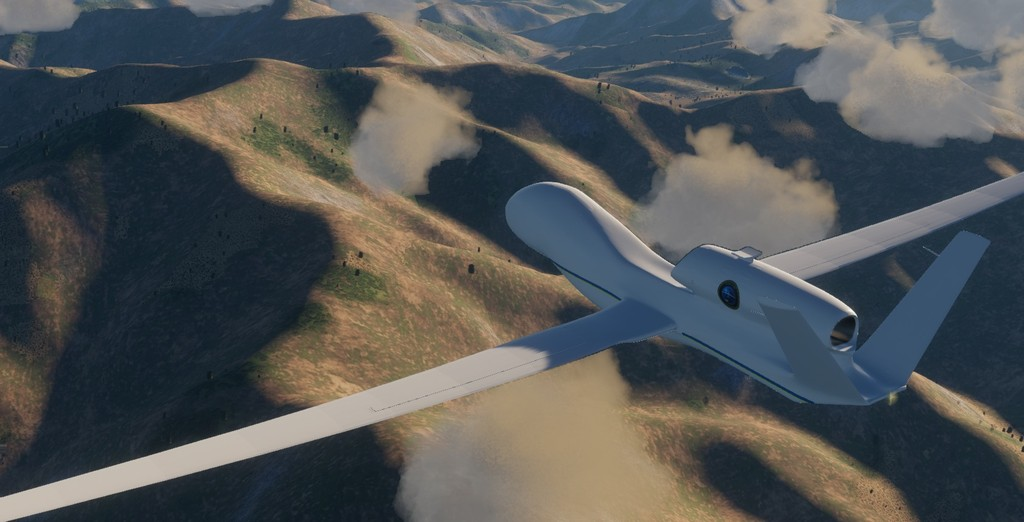
\includegraphics[width=0.8\textwidth]{aircraft.jpg}\par
\vspace{14mm}
\begin{minipage}{0.78\textwidth}\small
This manual describes the aircraft as simulated: its flight model, the laws that fly it, and the station it is commanded
from. The flight laws, the mission logic and the station are the simulation's own designs. The real aircraft's manuals
are not public, and none of this is the real aircraft's manual or procedures. The work is not connected with or
endorsed by NASA, Northrop Grumman or Rolls-Royce. The manual is generated with the aircraft: its tables of controls
and alerts, its limits and its performance figures come from the aircraft's own sources, so they follow it as it changes.
\end{minipage}
\vfill
{\small Generated from the aircraft's sources (\texttt{manual/} in its repository).\par}
\end{titlepage}

\chapter*{How to use this manual}
\addcontentsline{toc}{chapter}{How to use this manual}
The Global Hawk has no cockpit and nobody flies it. It is \emph{operated}: an operator tells it what is wanted, a
plan, ``go there'', ``hold'', ``come home'', and the aircraft works out how. This manual is for that operator. Read
Chapters~\ref{ch:general} and~\ref{ch:station}, then fly the first flight of Chapter~\ref{ch:normal} in the demo,
which needs nothing but the station's folder and a browser.

The parts are those of a flight manual: the system (Part~I), its limitations (Part~II), normal procedures (Part~III),
what the aircraft does by itself when things fail and what the operator does then (Part~IV), flying it by hand
(Part~V) and performance data (Part~VI). Words the screens show are set as \ann{Resume plan}; keys as \key{v}.

\paragraph{Warnings, cautions and notes.} Three kinds of notice stand apart from the text, by how much they matter:
\begin{warning}
A procedure or fact that, not heeded, may lose the aircraft.
\end{warning}
\begin{caution}
A procedure or fact that, not heeded, may end the flight's purpose.
\end{caution}
\begin{note}
A procedure or fact worth emphasising.
\end{note}

\paragraph{Its numbers.} Weights are pounds, speeds knots (KCAS, calibrated, unless stated), heights feet above sea
level. Performance is the flight model's, standard atmosphere, no wind; the comparisons with the real aircraft's
flight records that support it, and those that do not, are in the model's report.

\tableofcontents

\mainmatter
% =====================================================================================================================
\part{The system}
\chapter{General description}\label{ch:general}
\section{The aircraft}
The model is of the Global Hawk that NASA flew as N872NA, an RQ-4A: a wing of \MSpan\,ft span and \MWingArea\,ft$^2$,
one Rolls-Royce AE~3007H turbofan above the rear fuselage, flat rated at \MRating\,lbf, a V-tail whose two surfaces
work together as elevator and against each other as rudder, ailerons, spoilers, and a tricycle gear that retracts. It
is \MLength\,ft long. More than half of its take-off weight is fuel.
\begin{center}\small
\begin{tabular}{@{}lr@{}}
\toprule
Gross weight & \MGross\,lb \\
Empty & \MEmpty\,lb \\
Fuel, full: six tanks & \MFuel\,lb \\
Without fuel & \MNoFuel\,lb \\
Maximum height & \MMaxAlt\,ft \\
\bottomrule
\end{tabular}
\end{center}
It climbs at \MScheduleKcas\,KCAS to \MScheduleFrom\,ft and then at a Mach number that rises to \MScheduleMach{} at
\MScheduleTop\,ft, with the throttle at maximum, and above about 55\,000\,ft it goes on climbing only as it burns its
fuel: the cruise-climb. A flight to the end of its fuel lasts more than thirty hours.

\section{How it is flown}
The autonomy is on board. The aircraft carries a \emph{plan}: a taxi route, a take-off, a route of points with
heights, a landing, and a second route to fly if it stops hearing from the ground. Its flight laws hold attitude,
speed, height and track, steer it on the ground, rotate it, bring it down a glide path on its spoilers, flare it and
brake it. A mission manager gives the laws their next leg and nothing else. Four navigators supply its attitude, and
it votes between them.

The operator's station is a terminal. It shows what the aircraft says it is doing and sends commands, each of which
the aircraft checks and answers. The real aircraft is commanded the same way from two kinds of station: a launch and
recovery element near the runway, over a line-of-sight link, and a mission control element over a satellite, whose
link is slower. Here they are two names for the same page, \ann{LRE} and \ann{MCE}; the second has a delay of 1.2\,s
each way, an assumed figure.
\begin{warning}
Close the station's page, or lose its connection, and the aircraft takes it for a lost link: \MLinkTimeout\,s after
it last heard the station in control it leaves its plan, flies its lost-link route home and lands. (That is the time-out, which can be
set from the station: Section~\ref{sec:link}.)
\end{warning}

\section{What is the simulation's own}
The flight laws, the mission manager, the vote between navigators, the fuel system's layout, the station and the
head-up display are designs made for this simulation. They behave as public sources say the aircraft behaves, and the
model's performance is held to NASA's flight records, but none of them is the aircraft's own. Flying by hand
(Part~V) has no counterpart in the real aircraft at all.

% =====================================================================================================================
\chapter{The ground control station}\label{ch:station}
\section{Starting it}
The station is a page in a browser, in the aircraft's folder: \nolinkurl{GlobalHawk/gcs/index.html}. It can be used three
ways.
\begin{description}[leftmargin=8mm]
\item[The demo.] Open \texttt{index.html?demo=1}. The aircraft is then a stand-in inside the page that takes the same
commands and answers in the same words, with the real one's climb, descent and turn rates. It is not the flight
model. \texttt{\&speed=10} runs it ten times as fast. A strip under the top of the page can fail its engine or cut its
link. It has one station, no camera and no flying by hand.
\item[With FlightGear.] Start FlightGear with the aircraft and the option \texttt{-{}-httpd=5400}, at any airport,
then open \texttt{index.html}. If FlightGear runs on another machine, add its address:\\ \texttt{?host=\ldots\&port=5400}.
\item[With the flight model alone.] The command \texttt{python3 fdm/gcs\_server.py} stands in for\\ FlightGear; then open \nolinkurl{http://localhost:5400/gcs/}.
\end{description}
Add \texttt{\&station=MCE} (or any name) for a second crew position, and \texttt{\&latency=} in milliseconds to set
the link's delay.

\section{The page}
\begin{figure}[H]
\centering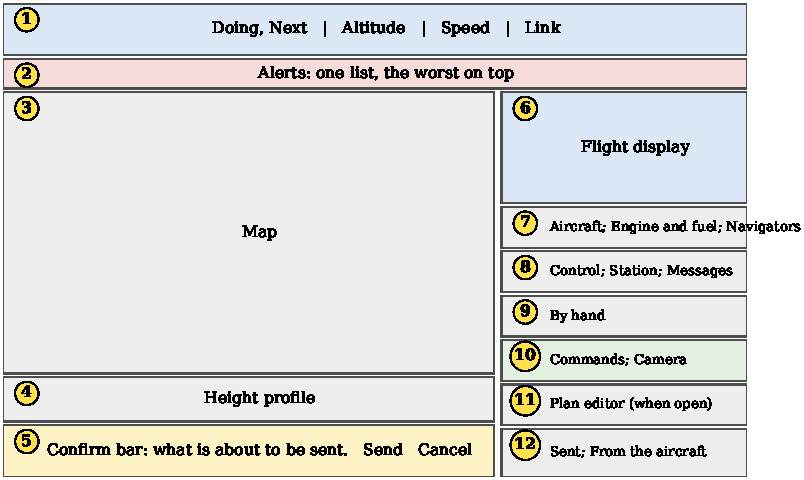
\includegraphics[width=0.9\textwidth]{layout.pdf}
\caption{The page.}\label{fig:layout}
\end{figure}
\begin{enumerate}
\item \emph{The strip.} \ann{Doing} and \ann{Next}: what the aircraft is doing now and what comes after, in its own
words. \ann{Altitude} and \ann{Speed}, each with the target the aircraft is flying towards. \ann{Link}: green with
the station's name when the aircraft is hearing this station; \ann{receiving only} when it shows the aircraft but is
not the station in control; \ann{NO LINK}. Beside it, the link's delay and what the aircraft will do if the link is lost: route home after a time-out. When the aircraft has gone three seconds without hearing the station in control, this note becomes a count: \ann{the aircraft has not heard this station for 12 s: route home in 18 s}.
\item \emph{Alerts} (Section~\ref{sec:alerts}).
\item \emph{The map} (Section~\ref{sec:map}).
\item \emph{The height profile}: the heights the plan asks for and the height forecast.
\item \emph{The confirm bar.} Every command is described here first, with what it will lead to, and goes to the
aircraft only on \ann{Send}.
\item \emph{The flight display} (Section~\ref{sec:pfd}).
\item \emph{Aircraft}: heading, Mach, ground speed, climb rate, fuel, throttle. \emph{Engine and fuel}: running or
failed, thrust, fuel flow, hours left at that flow, the six tanks. \emph{Navigators}: the four attitude sources,
each with a button that switches it off or on.
\item \emph{Control}: which station has control, and the handover (Section~\ref{sec:handover}). Under it, \emph{Station} and \emph{Messages} (Section~\ref{sec:link}).
\item \emph{By hand} (Part~V).
\item \emph{Commands} and \emph{Camera} (Sections~\ref{sec:commands} and~\ref{sec:camera}).
\item \emph{The plan editor}, when open (Section~\ref{sec:editor}).
\item \emph{Sent}: every command and its fate: sent, accepted, rejected with the aircraft's reason, or no answer.
\emph{From the aircraft}: its last notes.
\end{enumerate}
\begin{note}
A command counts only when the aircraft has answered it. \ann{Sent} says which have been.
\end{note}

\section{The map}\label{sec:map}
\begin{figure}[H]
\centering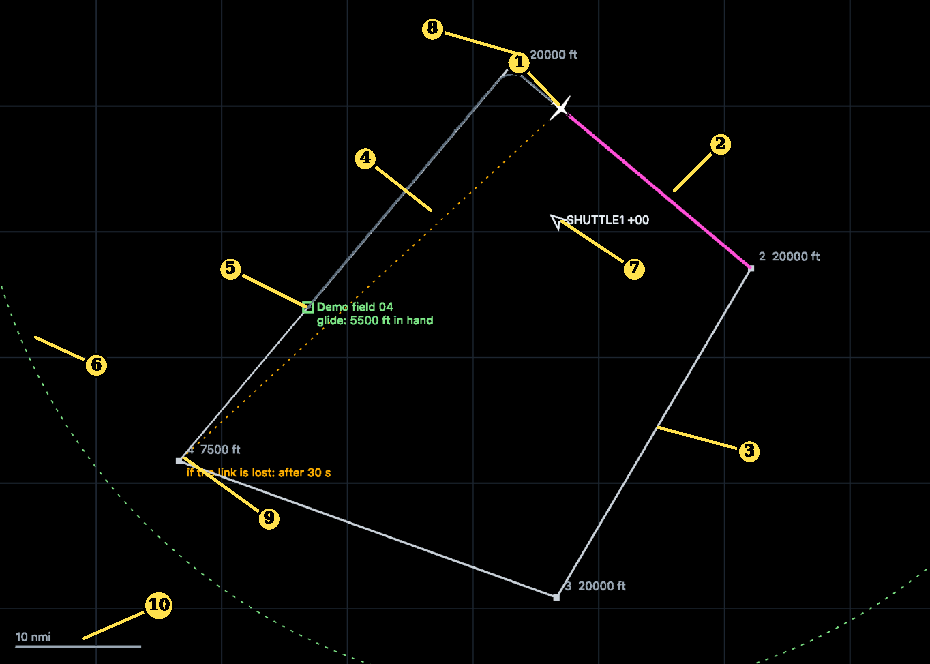
\includegraphics[width=0.92\textwidth]{map-turn.pdf}
\caption{The map, in the demo, on the second leg of a plan.}\label{fig:map}
\end{figure}
\begin{enumerate}
\item The aircraft, pointing along its heading, with its trail behind it.
\item The leg or hold being flown, magenta.
\item The plan as the aircraft holds it, white.
\item The lost-link route, amber and dashed, always drawn, with a line from the aircraft to its first point while
airborne.
\item A landing site, green, with the height the aircraft would have in hand there without its engine, or
\ann{OUT OF REACH}.
\item The glide reach: how far the aircraft's own planner would count on gliding.
\item Another aircraft: an arrowhead with its callsign and its height against ours in hundreds of feet.
\item A point of the route, with its number and height.
\item What the lost-link route is for, and after how long.
\item The scale. There is no background map: a grid and a scale.
\end{enumerate}
What is being prepared and has not been sent is drawn in blue dashes. The camera's target, when it is locked, is a
green cross with the line of sight. \ann{north up} turns the map so that the aircraft's track is at the top instead
(\ann{track up}), which is how a map is read when flying along it; the arrow in the corner always points to north.
\begin{center}\small\Tab{ctl_map}\end{center}

\section{The flight display}\label{sec:pfd}
\begin{figure}[H]
\centering
\begin{minipage}[c]{0.55\textwidth}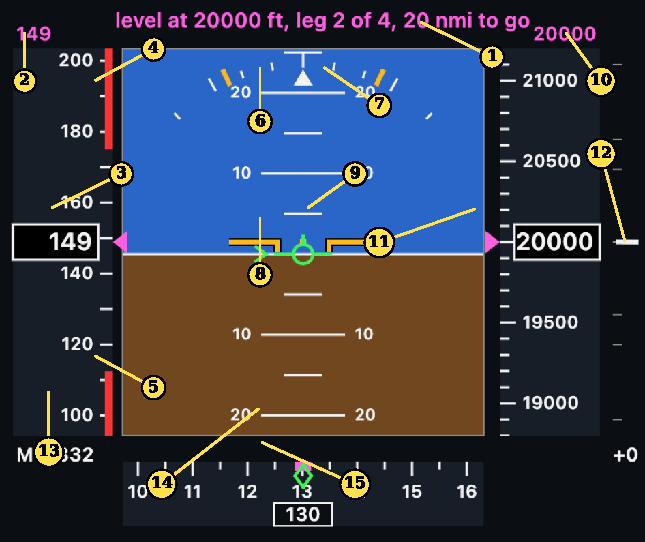
\includegraphics[width=\linewidth]{pfd-turn.pdf}\end{minipage}\hfill
\begin{minipage}[c]{0.42\textwidth}\small
\begin{enumerate}[leftmargin=*]
\item What the aircraft is doing.
\item The speed it is flying towards.
\item Speed, KCAS.
\item Red: faster than the aircraft may fly, Mach~\MFastMach or \MFastKcas\,KCAS.
\item Red: slower than it can fly, the angle-of-attack limit.
\item Bank scale; amber marks at the bank limit.
\item Bank pointer.
\item Flight path marker: where the aircraft is going. Its chevron is the acceleration along the path.
\item The aircraft's nose.
\item The height it is flying towards.
\item Height, ft.
\item Vertical speed.
\item Mach number.
\item Heading, with the track (green) and the leg's course (magenta).
\item Heading in figures.
\end{enumerate}
\end{minipage}
\caption{The flight display.}\label{fig:pfd}
\end{figure}
The two red bands are where the aircraft cannot fly. High up they close in on each other. The speed and height tapes carry a trend arrow, where the value will be in 10\,s.
The aircraft keeps itself between the bands; the display is there so that the operator can see how near it is.

\section{Alerts}\label{sec:alerts}
One list under the strip, the worst on top: warnings red, cautions amber, advisories plain. Each says what it is and
what to do. The aircraft raises them, so every station sees the same list; the station adds only the loss of its own
link and traffic. A tone sounds for a new warning or caution until \ann{OK} is pressed on it. A browser gives no sound
until the page has been clicked once.
\begin{center}\small\Tab{alerts}\end{center}

\section{Commands}\label{sec:commands}
\begin{center}\small\Tab{ctl_commands}\end{center}
\begin{center}\small\Tab{ctl_confirmingacommand}\end{center}
The aircraft refuses a command it cannot do, and says why: a go-to or a hold on the ground or while landing, a height
outside 0 to \MMaxAlt\,ft, a start with no plan or a second start, a resume when it is on its plan. It refuses any
command from a station that does not have control, naming the one that has.

A plan is a file: a field, items (taxi, take-off, route, landing, hold), a lost-link route that begins with a route
and ends in a landing, and landing sites for a glide without the engine. The aircraft refuses a plan with an unknown
item, a point off the earth, a height outside its range, a leg over \MMaxLeg\,nmi, a take-off not followed by a
route, or a landing whose fix is less than \MMinFinal\,nmi out.

\section{The plan editor and the forecast}\label{sec:editor}
\ann{Edit plan} takes the plan the aircraft holds. Choose \ann{Route} or \ann{Lost-link route}; click the map to add a
point after the selected one, drag a point to move it, type a height, $\times$ to delete one. Taxi, take-off and
landing are kept as they came. Nothing is sent until \ann{Send plan\ldots} and then \ann{Send}. Sent while the
aircraft is enroute, the plan is taken from its first route on, and the aircraft turns onto it at once.
\begin{center}\small\Tab{ctl_planeditor}\end{center}
While a plan is edited, a table gives for each point the leg's length and the \emph{forecast}: the time, the fuel left
there, and whether the height asked for is reached by then. Under it: the time, fuel and distance of the whole, and
the landing: its weight, where it touches down, where the rollout ends and how much runway to have. The check the
aircraft will make of the plan runs here first, so a fault shows before sending. \ann{Go to\ldots} and \ann{Return
home} show a forecast in the confirm bar too.
\begin{note}
The forecast is for a standard atmosphere, with no wind and no turns. Against flights of the flight model it was
within 3\,\% in time and fuel. The aircraft does not use it.
\end{note}

\section{Control and handing over}\label{sec:handover}
Each page opened with its own station name is a crew position. The aircraft decides who has control: the first
station it hears. The others watch: the same map and alerts, their commands greyed. The lost-link watch follows the
station in control, not the watchers.
\begin{center}\small\Tab{ctl_control}\end{center}

\section{The link, this station and messages}\label{sec:link}
\paragraph{The time-out.} \ann{Link time-out\ldots} sets how long the aircraft may go without hearing the station in
control before it leaves its plan for the lost-link route: \MLinkTimeout\,s unless it has been set, and the aircraft
takes \MLinkTimeoutMin{} to \MLinkTimeoutMax\,s. Only the station in control may set it; like any command it is
shown in the confirm bar and counts when the aircraft answers. The bounds are assumed: under \MLinkTimeoutMin\,s a
satellite delay and one missed heartbeat could trigger the loss.
\begin{caution}
A short time-out sends the aircraft home on a brief break in the link. A long one lets it fly on for minutes with
nobody commanding it. Set it for the link in use.
\end{caution}
\paragraph{When the link goes and when it comes back.} After three seconds without an uplink from the station in
control, the strip counts down to the lost-link route. When the link is lost, \ann{NO LINK TO THE AIRCRAFT} (at the
station that lost it) or \ann{LINK WAS LOST} (from the aircraft, to every station) is raised with a two-note tone that no
other alert uses, repeating until it is acknowledged. When the link comes back \ann{LINK RESTORED} stands for twenty
seconds; if the aircraft is still on its lost-link route it says so, and says to \ann{Resume plan} to go on.
\paragraph{Closing the page.} A station that has control of a flight is asked before its page is closed, because
closing it cuts the link. A station that is only watching may close its page.
\begin{center}\small\Tab{ctl_station}\end{center}
The delay is what this station's link adds each way to commands and to what comes down. It can be changed while the
page runs; it takes effect on the next message. \ann{Answer time} is measured: how long the aircraft took to answer
the last commands, so it is about twice the delay plus the aircraft's own time. \ann{Last heard} is how long ago anything
came down from the aircraft.
\paragraph{Messages.} A line typed under \ann{Messages} goes to every other station at once, and is shown with who sent
it and when it arrived. It is text, between the stations of this aircraft only; it is not delayed by the link's delay, as
the crews of a real aircraft would talk by voice, and the aircraft does not see it. A new message from another station
sounds once and the heading says how many are new. The demo has one station and no messages.
\begin{center}\small\Tab{ctl_messages}\end{center}

\section{The belly camera}\label{sec:camera}
The \ann{Camera} panel is the sensor operator's. Its commands are not flight commands: they need no control of the
aircraft and get no answer, and they arrive late by the link's delay like everything else. What the camera is locked
on is written in the panel and drawn on the map.
\begin{center}\small\Tab{ctl_camera}\end{center}
The arrows move a locked point only while FlightGear is showing the belly camera's view.

% =====================================================================================================================
\chapter{The aircraft in FlightGear}
\section{Views}
\key{v} steps through the views. The first is the \ann{Nose Camera}, looking ahead from the nose with the head-up
display; \ann{Belly Camera} is the sensor operator's, in the dome under the fuselage; the others are FlightGear's
outside views. \key{x} and \key{X} zoom. \key{h} switches the head-up display.

\section{The head-up display}
\begin{figure}[H]
\centering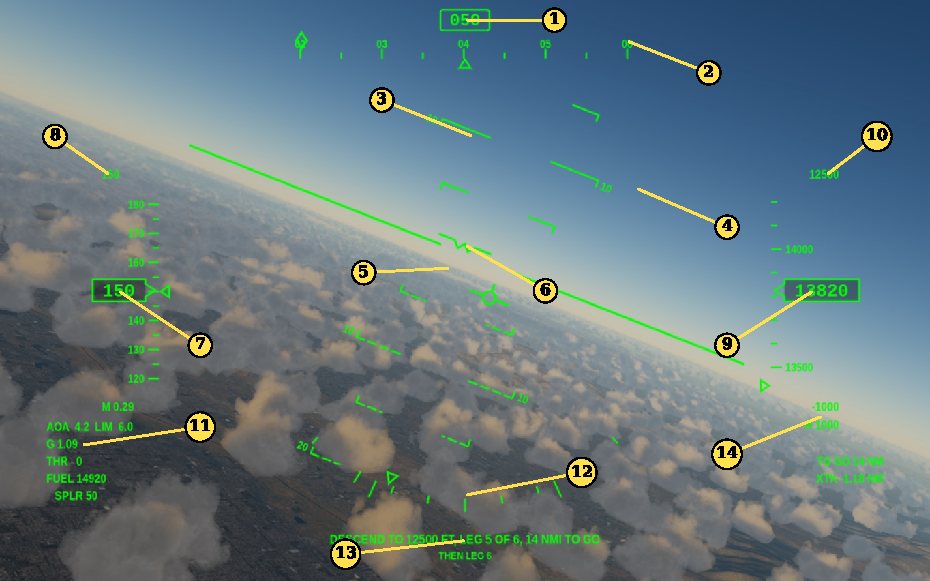
\includegraphics[width=0.95\textwidth]{hud.pdf}
\caption{The head-up display over the nose camera's picture, in a turn.}\label{fig:hud}
\end{figure}
\begin{enumerate}
\item Heading.
\item Heading scale, with a diamond at the heading or course the laws are flying to.
\item Pitch ladder, every 5$^\circ$; it lies on the outside world.
\item Horizon line: it lies on the horizon.
\item Flight path marker: where the aircraft is going.
\item The aircraft's nose.
\item Speed, KCAS, on its scale.
\item The speed the laws are flying to.
\item Height, ft, on its scale.
\item The height the laws are flying to.
\item Mach; angle of attack and its limit; load factor; throttle; fuel.
\item Bank scale and pointer.
\item What the aircraft is doing, and under it what the operator must know.
\item Climb rate, and height above the ground.
\end{enumerate}
It shows what the aircraft's laws have. Nothing on it flies the aircraft.

\section{The belly camera's picture}
\begin{figure}[H]
\centering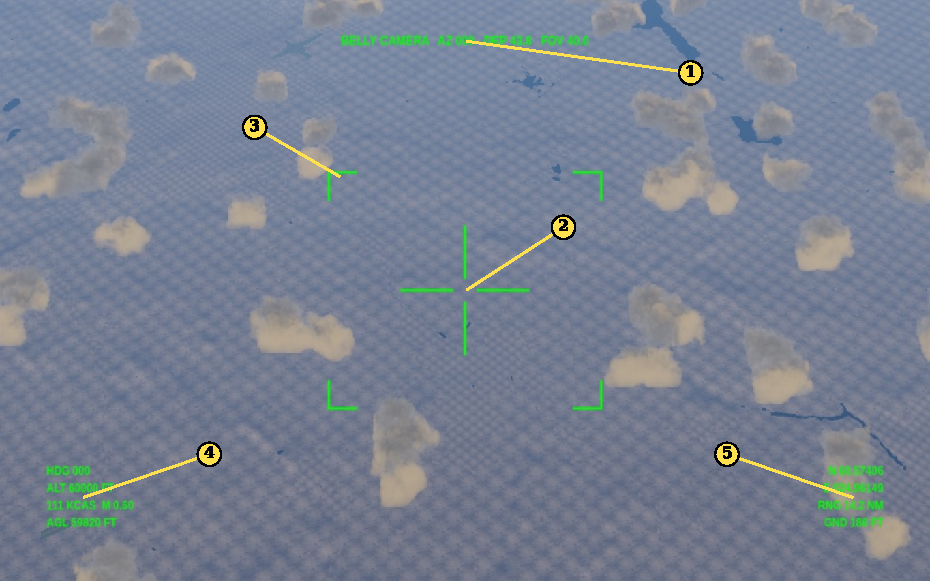
\includegraphics[width=0.95\textwidth]{belly.pdf}
\caption{The belly camera's picture.}\label{fig:belly}
\end{figure}
\begin{enumerate}
\item Where the camera looks: azimuth, depression below the horizon, field of view.
\item The cross.
\item The frame; its corners close to a box when the camera is locked.
\item The aircraft: heading, height, speed and Mach, height above the ground.
\item What is under the cross: latitude and longitude, slant range, the ground's height there.
\end{enumerate}
Locked, the camera is turned every frame to look at a point of the ground or at a moving object: any aircraft, ship
or vehicle FlightGear has. With the belly camera's view up and the aircraft flying itself, the stick turns the
camera; locked on a point, it moves the point. The horizon is kept level in the picture as the aircraft banks, unless
switched off.

\section{The aircraft's menu}
\begin{center}\small\Tab{ctl_theaircraftsmenuinflightgear}\end{center}
\begin{center}\small\Tab{ctl_thecamerasdialog}\end{center}

\section{Starting in the air}
Started in the air, the aircraft is held still for about two seconds while FlightGear's wind settles, then set on its
own level trim for the height and speed asked for, and flies on, holding them. With no speed given it takes the
speed of its schedule for that height.
\begin{note}
With full tanks the aircraft cannot fly level above about 50\,000\,ft. Started higher, it starts with the fuel it
could have left there, and says so. A speed it cannot fly at that height is changed to the nearest it can.
\end{note}
High up, the aircraft widens FlightGear's terrain range with its height, so that the ground runs towards the horizon;
expect more scenery to be loaded. The menu switches it off.

\section{Sounds}
The sounds are synthesised from the engine's and the airframe's physics, not recorded. In the two cameras' views
they are what a microphone in the nose bay would hear; in the outside views, the aircraft from where the viewer stands.

% =====================================================================================================================
\part{Limitations}
\chapter{Operating limitations}
The aircraft keeps these itself in automatic flight and in the protected law. They are the simulation's: none is a
published limit of the real aircraft except the maximum height and the weights.
\begin{center}\small
\begin{tabularx}{\textwidth}{@{}>{\raggedright\arraybackslash}p{52mm}>{\raggedright\arraybackslash}X@{}}
\toprule
Maximum height & \MMaxAlt\,ft. A plan point or a commanded height above it is refused. \\
Speed, upper & \MFastKcas\,KCAS or Mach~\MFastMach, whichever is lower: above it the laws raise the nose. \\
Speed, lower & The angle-of-attack limit: \MAlphaLow$^\circ$ at low Mach numbers, falling to \MAlphaCruise$^\circ$ at Mach~0.6. \\
Bank & \MBankLow$^\circ$ up to \MBankLowTo\,ft, falling to \MBankHigh$^\circ$ from \MBankHighFrom\,ft. Turns are flown at \MBankCmd\,\% of it. \\
Hold & Circles to the right at \MHoldBank$^\circ$ of bank. \\
Approach & A \MGlideDeg$^\circ$ glide path at idle thrust, at the speed for a lift coefficient of \MApproachCl{} at the weight; the landing's fix at least \MMinFinal\,nmi out. \\
Lost link & \MLinkTimeout\,s without the station in control, unless set (\MLinkTimeoutMin{} to \MLinkTimeoutMax\,s, Section~\ref{sec:link}). \\
Fuel & \ann{FUEL LOW} below \MFuelLow\,lb. \\
Structure (assumed) & Load factor \MNzMin{} to $+$\MNzMax; \MLimitKeas\,KEAS; Mach~\MLimitMach. Passing one raises \ann{STRUCTURAL LIMIT PASSED}. \\
Wind, weather & None is allowed for anywhere: no check of the model or the laws was flown in wind, turbulence or icing. \\
\bottomrule
\end{tabularx}
\end{center}
\begin{caution}
A landing soon after take-off is a heavy one and needs almost twice the runway of a landing at the end of a long
flight (Chapter~\ref{ch:perf}). The aircraft does not know its runway's length: it lands where the plan tells it.
\end{caution}

% =====================================================================================================================
\part{Normal procedures}
\chapter{Normal procedures}\label{ch:normal}
\section{A first flight, in the demo}
\begin{enumerate}
\item Open \texttt{index.html?demo=1\&speed=10}. \ann{Link}: \ann{LRE linked}. \ann{Doing}: \ann{no plan}.
\item \ann{Demo plan}. The plan is drawn in blue dashes; the confirm bar describes it. Nothing has been sent.
\ann{Send}. The plan turns white, the lost-link route amber: the aircraft holds it now.
\item \ann{Start}, \ann{Send}. The aircraft taxis out, takes off and flies the route. \ann{Doing} and \ann{Next} say
so as it goes.
\item Enroute: \ann{Go to\ldots}, click the map, set a height, read the forecast in the confirm bar, \ann{Send}. The
aircraft leaves its plan, flies to the point and holds over it; \ann{OFF THE PLAN} stands in the alert list.
\item \ann{Altitude\ldots}, a height, \ann{Send}: the hold's height changes.
\item \ann{Resume plan}, \ann{Send}: back to the leg that was left.
\item \ann{Edit plan}: add a point, change a height, read the forecast, \ann{Send plan\ldots}, \ann{Send}.
\item \ann{Cut the link} on the demo strip. After \MLinkTimeout\,s the aircraft leaves for home by itself.
\end{enumerate}

\section{With FlightGear}
\begin{enumerate}
\item Start FlightGear with the aircraft on a runway, with \texttt{-{}-httpd=5400}. The engine is running; the
aircraft stands on its brakes.
\item Open the station. \ann{Link}: \ann{LRE linked}.
\item \ann{Plan from here}, \ann{Send}: a local flight from the runway the aircraft stands on.
\item In the editor, type how much runway there is past the aiming point, if known, and read the landing's forecast.
\item \ann{Start}, \ann{Send}.
\end{enumerate}
\begin{note}
A plan's start is refused with the engine off. \ann{Autostart} in the aircraft's menu starts it.
\end{note}
\begin{caution}
Open the station after FlightGear has finished loading, or leave it open: either way works. The demo plan is for the
made-up field of the demo, not for FlightGear's airports.
\end{caution}

\section{Enroute}
The aircraft needs nothing from the operator to fly its plan. What the operator does is watch three things: \ann{Doing}
and \ann{Next} against what was intended; the alert list; and the amber route, which is what will happen if the
station falls silent. Keep the lost-link route current as the flight moves on: edit it and send it.

\section{Handing over control}
\begin{enumerate}
\item The station in control: tick the three checks under \ann{Control}, choose the station, \ann{Offer control}.
\item The station offered to: tick its own three checks, \ann{Accept control}. Control passes at that moment.
\item An offer not accepted lapses after \MOfferSec\,s; \ann{Withdraw the offer} takes it back sooner.
\end{enumerate}
The checks are the handover's briefing: that both stations show the same plan and position, that the aircraft's state
and alerts have been told, that no command is waiting for an answer, and that the receiving operator knows the
station's link delay. The briefing itself goes in \ann{Messages}.

\section{Landing}
The aircraft lands by itself at the end of its plan or of its lost-link route: level in the landing configuration
until the glide path comes down to it, then down the path on its spoilers at idle thrust, a flare at \MFlareHeight\,ft
of wheel height, and brakes held to \MDecel\,$g$ on the runway. It touches down 800 to 1200\,ft past the plan's
aiming point, further when heavy (Chapter~\ref{ch:perf}). Before \ann{Return home}, read the landing's forecast in the confirm bar.

% =====================================================================================================================
\part{Abnormal procedures}
\chapter{When things fail}
In each case the aircraft acts first and by itself. The operator's part is to understand what it has done and to
decide what comes next.

\section{The link is lost}
\emph{The aircraft:} after the time-out (\MLinkTimeout\,s unless set) without hearing the station in control, leaves its plan for the lost-link
route and lands at its end. It raises \ann{LINK WAS LOST} and stays on that route even when it hears a station again.
Before that the strip counts down to it.

\emph{The operator:}
\begin{enumerate}
\item At the station that lost the link, \ann{NO LINK TO THE AIRCRAFT}: restore the connection.
\item When \ann{Link} is green again, \ann{LINK RESTORED} says so. Read \ann{Doing}: the aircraft is on its lost-link route.
\item To go on with the mission: \ann{Resume plan}, \ann{Send}. To let it come home: nothing.
\item If the station in control cannot be restored, another station may \ann{Take control}.
\end{enumerate}

\section{The engine fails}
\emph{The aircraft:} chooses the landing site it can reach with the most height to spare, counting on a glide of
\MGlideRatio{} to 1, \MTurnCost\,ft for every 90$^\circ$ of turn and \MInHand\,ft in hand, glides to it, circles over a
point on the approach to lose what height it has too much, and lands. It raises \ann{ENGINE FAILED} and names the site.

\emph{The operator:}
\begin{enumerate}
\item Read which site it has chosen. Clear that runway.
\item Nothing else: \ann{Resume plan} is refused with the engine failed. No restart is modelled.
\end{enumerate}
\begin{warning}
With \ann{NO RUNWAY IN REACH} the aircraft glides towards the nearest site and will not reach it. A landing off a
runway is not built. Watch the glide reach on the map in flight, and plan landing sites along the route.
\end{warning}

\section{The navigators}
\emph{The aircraft:} with three or four navigators on, it takes the middle attitude; with two, their mean while they
agree within 3$^\circ$, and otherwise the one whose bank agrees with its turn rate. A disagreement raises
\ann{NAVIGATORS DISAGREE}.

\emph{The operator:}
\begin{enumerate}
\item \ann{NAVIGATORS DISAGREE}: land. Switch off the one that is wrong only if it is known which.
\item \ann{ONE NAVIGATOR LEFT}: switch another on under \ann{Navigators}.
\end{enumerate}
\begin{warning}
Two navigators that are wrong the same way are not caught: the aircraft follows them, and no alert is raised. Fly
with three or four on.
\end{warning}

\section{Other alerts}
\ann{FUEL LOW}: \ann{Return home}. \ann{ANGLE OF ATTACK LIMIT}: the aircraft is holding itself at the limit; it has
been asked for more height or less speed than it has the performance for there. \ann{STRUCTURAL LIMIT PASSED}: land.
\ann{TRAFFIC}: change height or route; the station suggests no manoeuvre.

% =====================================================================================================================
\part{Flying by hand}
\chapter{Flying by hand}
The real aircraft has no stick. This is the simulation's addition, so that the aircraft can be flown in FlightGear
with a joystick, and from the station through the link's delay, which shows why nobody does.

\section{From the station}
Enroute, the station in control chooses \ann{Protected} or \ann{Direct} under \ann{By hand}, confirmed like any command.
\begin{center}\small\Tab{ctl_byhand}\end{center}
A gamepad is used if one is connected: left stick pitch and roll, right stick pedals, triggers throttle, bumpers
spoilers. Otherwise the keys: arrows for the stick (up is stick forward), \key{Q} and \key{E} pedals, \key{W} and
\key{S} throttle, \key{Z} and \key{X} spoilers.

\emph{Protected.} Fore and aft, the stick asks for a pitch rate, up to \MManualPitchRate$^\circ$/s, and the aircraft
holds the attitude when it is released. Sideways it asks for a bank angle, wings level when released. The pedals ask
for sideslip, up to \MManualBeta$^\circ$. The aircraft keeps its limits of angle of attack, speed and bank.

\emph{Direct.} The surfaces follow the stick, with rate damping only.
\begin{warning}
The direct law has no limits. The aircraft can be stalled, oversped and overstressed in it.
\end{warning}
\begin{caution}
With a link delay, what is seen is that much old and what is done arrives that much late. With the 1.2\,s of the
\ann{MCE} station, height cannot be held closely by hand.
\end{caution}
If the link is lost while the aircraft is flown by hand, it goes back to automatic by itself and flies its lost-link
route.

\section{In FlightGear}
On the ground before a plan is started, and whenever a joystick is used with no station in control, the aircraft is
flown through the protected law: the stick, pedals and throttle lever of FlightGear.

% =====================================================================================================================
\part{Performance data}
\chapter{Performance data}\label{ch:perf}
All of it is the flight model's, standard atmosphere, no wind, sampled for the station's forecast, which uses these
same tables.

\section{Speeds}
The schedule's true airspeed by height:
\begin{center}\small\Tab{perf_speed}\end{center}

\section{Climb}
Rate of climb at maximum thrust on the schedule, ft/min. A dash: the aircraft cannot climb there at that weight.
\begin{center}\small\Tab{perf_climb}\end{center}
Fuel flow in that climb, lb/h:
\begin{center}\small\Tab{perf_climbfuel}\end{center}

\section{Level flight}
Fuel flow in level flight on the schedule, lb/h. A dash: the aircraft cannot hold that height at that weight.
\begin{center}\small\Tab{perf_level}\end{center}

\section{Descent}
Rate of descent at idle thrust with half spoilers, as the aircraft descends, ft/min:
\begin{center}\small\Tab{perf_descent}\end{center}

\section{Landing}
Feet past the plan's aiming point: where the aircraft touches down, where the rollout ends (15\,kt, where the taxi
begins), and the runway to have past the aiming point, which is the rollout with 15\,\% in hand, an assumed allowance.
A dry, level runway.
\begin{center}\small\Tab{perf_landing}\end{center}

% =====================================================================================================================
\appendix
\chapter{The station against a list of what a remote pilot station needs}\label{app:hl}
Hobbs and Lyall's \emph{Human Factors Guidelines for Remotely Piloted Aircraft System Remote Pilot Stations} (NASA,
2016) lists \MHlAll{} guidelines: tasks the station must make possible (T), information it must give (I), controls
(C) and properties of its displays (P). The table holds every one against the station as it is: \MHlMet{} met,
\MHlPartly{} partly, \MHlNot{} not met, \MHlNa{} that do not apply to a simulation with one simulated link, no radio
and no flight termination system. The guidelines are shortened here; the study has their full wording.

What it shows: the station does what the guidelines ask about the lost-link route (always drawn and distinguishable, its
time-out shown, set from the station and counted down), about who has control and handing it over (with messages between
the crews), and about consumables. About the link itself it can only do what the simulated link has: it is there or it is
not, so nothing about its strength, coverage, interference or choice. It has no map behind its grid, no airspace or
weather, no radio or air traffic control, and no flight termination. The guidelines that were not met and could have been
are those that need data this simulation does not have, not ones left undone.
\par
{\footnotesize\begin{longtable}{@{}>{\raggedright\arraybackslash}p{12mm}>{\raggedright\arraybackslash}p{57mm}>{\raggedright\arraybackslash}p{13mm}>{\raggedright\arraybackslash}p{70mm}@{}}
\toprule
\textbf{Code} & \textbf{Guideline} & \textbf{Status} & \textbf{In the station} \\
\midrule
\endhead
\addlinespace\multicolumn{4}{@{}l}{\textbf{Aircraft systems and automation}} \\
T\_1.1.1 & If an on-board camera is used for flight control tasks, the RPS should enable the pilot to align the camera with the longitudinal access of the\ldots{} & \textbf{met} & The nose camera is fixed on the aircraft's axis; the belly camera is not used to fly. \\
T\_1.1.2 & If an on-board camera is used for flight control tasks, the RPS should enable the pilot to align the camera with the longitudinal access of the\ldots{} & \textbf{met} & As T\_1.1.1 (the study lists it twice). \\
P\_1.1.1 & Not enable the pilot to disengage automation in flight if the aircraft will depart from controlled flight as a result & partly & Protected keeps the aircraft inside its limits. Direct has none and is offered all the same, enroute only: a simulator's choice. \\
P\_1.1.2 & Prevent multiple operators from operating the same application or procedure at any one time & \textbf{met} & One station has control; another's commands and stick are refused by the aircraft, naming who has it. \\
P\_1.1.3 & It should be possible to set an RPS to a receive only mode, in which the RPS displays information downlinked from an RPA in the absence of an active\ldots{} & \textbf{met} & A station without control shows everything and its commands are greyed: Link reads ''receiving only''. \\
\addlinespace\multicolumn{4}{@{}l}{\textbf{Consumables}} \\
T\_1.2.1 & Monitor the status of consumable resources & \textbf{met} & Engine and fuel: fuel, flow, hours left at that flow, six tanks. \\
I\_1.2.1 & Information on the status of consumable resources & \textbf{met} & As T\_1.2.1; FUEL LOW is raised by the aircraft; the forecast gives fuel at each point and on landing. \\
\addlinespace\multicolumn{4}{@{}l}{\textbf{The station itself}} \\
T\_1.3.1 & Perform checks on the status of RPS systems & partly & Only the link's state and the connection line at the foot of the page; a gamepad is named when one is found. \\
T\_1.3.2 & Perform a pre-flight check on an alternate control station, or confirm that this check has been performed & \emph{not met} & Nothing checks another station before a handover beyond its being heard. \\
T\_1.3.3 & Monitor the performance of RPS support services, e.g. air conditioning and electrical power & -- & A browser page has no support services to watch. \\
I\_1.3.1 & Health and status information on the RPS & partly & As T\_1.3.1. \\
\addlinespace\multicolumn{4}{@{}l}{\textbf{The link}} \\
T\_1.5.1 & Confirm spectrum availability before selecting link & -- & One simulated link; no spectrum. \\
T\_1.5.2 & Select the appropriate communication mode (e.g. terrestrial/satellite, frequency) & partly & The station's name and delay are chosen in the page's address (LRE: none; MCE: 1.2 s), not while running. \\
T\_1.5.3 & Maintain awareness of selected communication mode & \textbf{met} & Link shows the station's name and its delay. \\
T\_1.5.4 & Confirm that communication link is effective, and established with the correct UA & partly & Link turns green only when the aircraft is hearing this station, and every command is answered. There is one aircraft, so ''the correct one'' is not shown. \\
T\_1.5.5 & Identify if more than one control station is linked with the UA & \textbf{met} & Control lists the stations the aircraft hears and which has control. \\
T\_1.5.6 & Maintain awareness of link strength, or link abnormalities & \emph{not met} & Link strength is not modelled: the link is there or it is not. \\
T\_1.5.7 & Maintain awareness of link latency, where relevant & \textbf{met} & The delay is shown beside Link, in seconds. \\
T\_1.5.8 & Anticipate link degradations or diminished link strength & \emph{not met} & No link coverage is modelled. \\
T\_1.5.9 & Maintain an awareness of the geographic limits of the link and potential obstructions to signal & \emph{not met} & No link coverage is modelled. \\
T\_1.5.10 & Maintain awareness of crew actions or control inputs that could interrupt or degrade the link & partly & Closing the page is the one crew action that cuts the link, and the manual and the page say what follows. \\
T\_1.5.11 & Respond to interference with the signal, (e.g. other users of frequency, jamming attempts) & -- & No interference is modelled. \\
T\_1.5.12 & Change the link during flight operations as necessary & \emph{not met} & The link cannot be changed in flight; control can be handed to a station on another link. \\
T\_1.5.13 & Assess link strength and quality before switching link & \emph{not met} & As T\_1.5.6. \\
T\_1.5.14 & Define the duration of a loss of link that must occur before the lost link alert is activated, or the RPA enters its lost link procedure & \emph{not met} & The 30 s is shown, not set from the station (it is the flight model's ap/link-timeout-sec). \\
T\_1.5.15 & Manage resumption of the signal after a lost link & \textbf{met} & LINK WAS LOST stands until Resume plan; the aircraft stays on its lost-link route until told. \\
I\_1.5.1 & Predictive information on the quality and strength of a C2 link before the link is actively used to control the UA & \emph{not met} & No link quality is modelled. \\
I\_1.5.2 & Identify which C2 link settings are active (e.g. selected frequency, satellite vs terrestrial) & partly & Station name and delay; nothing else to set. \\
I\_1.5.3 & Information to confirm that effective control is established with the correct UA & partly & As T\_1.5.4. \\
I\_1.5.4 & Information on the geographic limits of the link & \emph{not met} & No link coverage is modelled. \\
I\_1.5.5 & Information on spectrum activity from a spectrum & -- & No spectrum is modelled. \\
I\_1.5.6 & Alert the pilot when the RPA is approaching an area where link is likely to be lost & \emph{not met} & No link coverage is modelled. \\
I\_1.5.7 & Alert the pilot when the link is lost & \textbf{met} & NO LINK TO THE AIRCRAFT at the station that lost it; LINK WAS LOST from the aircraft to every station that hears it. \\
I\_1.5.8 & The RPA will transmit a pre-determined transponder code when the link is lost & \emph{not met} & No transponder is modelled. \\
I\_1.5.9 & Monitor the strength of the link & \emph{not met} & As T\_1.5.6. \\
I\_1.5.10 & Alert the pilot whenever the C2 link experiences interference, whether resulting from natural phenomena, payload or other equipment associated with\ldots{} & -- & No interference is modelled. \\
I\_1.5.11 & Display to the pilot the source of downlink transmissions & partly & One aircraft; the connection line names the address the telemetry comes from. \\
I\_1.5.12 & Where relevant, the RPS should provide the pilot with information on link latency, in milliseconds & partly & The delay set for the station is shown in seconds; it is not measured. \\
I\_1.5.13 & Anticipate link degradations or diminished link strength. This information may include link footprint, including areas that may be affected by\ldots{} & \emph{not met} & No link coverage is modelled. \\
I\_1.5.14 & Manage link security & \emph{not met} & No link security: anything that reaches FlightGear's web server can command the aircraft. \\
I\_1.5.15 & Inform the pilot when a lost link is resumed & partly & Link turns green again and NO LINK clears; no separate message says it. \\
C\_1.5.1 & Select the communication mode (e.g. terrestrial/satellite, frequency, transmission power) & partly & As T\_1.5.2. \\
C\_1.5.2 & A control to enable the pilot to request a link status report & \emph{not met} & No such control; the link's state is always shown. \\
C\_1.5.3 & If antenna selection is performed by the pilot, then the RPS should support an external command to set the antenna used for communication & -- & No antennas. \\
C\_1.5.4 & Set the duration of a link outage that must occur before a lost link response is triggered & \emph{not met} & As T\_1.5.14. \\
P\_1.5.1 & There must be an alert for the UAS [RPAS] crew, via a clear and distinct aural and visual signal, for any total loss of the command and control data\ldots{} & \textbf{met} & NO LINK TO THE AIRCRAFT is a warning at the top of the list, with the warning tone. \\
P\_1.5.2 & The aural warning for lost control link should be a unique sound, not also used to signify other conditions & \emph{not met} & The warning tone is the same for every warning. \\
P\_1.5.3 & The maximum range of the C2 datalink (datalink footprint) for all altitudes and directions relative to the signal source should be presented visually\ldots{} & \emph{not met} & No link footprint. \\
P\_1.5.4 & Areas where the C2 link (datalink footprint) are predicted to be masked by terrain should be displayed on the C2 datalink display & \emph{not met} & No link footprint. \\
P\_1.5.5 & If the datalink footprint can be suppressed, it should be automatically displayed when the RPA is approaching a location where a loss of link is\ldots{} & \emph{not met} & No link footprint. \\
P\_1.5.6 & The C2 datalink footprint should be easily distinguishable from other footprints that may be present on the operator map display & \emph{not met} & No link footprint. \\
P\_1.5.7 & If the payload utilizes a link separate to the aircraft control link, any display of payload link quality should be separate and clearly\ldots{} & -- & The camera has no link of its own: its commands go the way of the others. \\
P\_1.5.8 & If an aural warning is used to indicate loss of payload link, the sound should be dissimilar to that used to indicate loss of control link & -- & As P\_1.5.7. \\
P\_1.5.9 & Security features designed to prevent unapproved access (logon and logoff functions) should not result in inadvertent lockouts of authorized\ldots{} & -- & No log-on. \\
P\_1.5.10 & The RPS, in combination with the other elements of the RPAS should comply with control link latency (time from initiation of a maneuver to a\ldots{} & partly & By hand with no delay the stick reaches the surfaces in a frame; with the satellite delay it does not meet a manned aircraft's figure, which is the point made. \\
\addlinespace\multicolumn{4}{@{}l}{\textbf{Handing over control}} \\
T\_1.6.1 & Enable control to be transferred between a giving and receiving RPS in a manner that is seamless and transparent to ATC & -- & No air traffic control is simulated. \\
T\_1.6.2 & Enable continuity of pilot function to be maintained during the transfer of control between a giving and receiving RPS & \textbf{met} & The aircraft goes on flying its plan through a handover; control passes at the acceptance. \\
T\_1.6.3 & Ensure that operating parameters are identical before and after handover & partly & Both stations show the plan and state the aircraft sends, so they cannot differ; each pilot ticks that they have compared them. \\
T\_1.6.5 & In cases where more than one RPS could be linked with the RPA, each RPS will enable the pilot to monitor which entity has control of the aircraft and\ldots{} & \textbf{met} & Control: who has it, to whom it is offered, which stations are heard. \\
T\_1.6.6 & Enable the giving and receiving pilots to confirm that control settings are appropriate and consistent before a handover is accomplished & \textbf{met} & Three ticks on each side before the offer and before the acceptance. \\
T\_1.6.7 & Enable the receiving pilot to monitor the status of the RPA by receiving telemetry from the RPA before establishing control of the UA & \textbf{met} & A watching station has the whole picture before it accepts. \\
T\_1.6.8 & Facilitate a handover briefing between the giving and receiving pilots & partly & The ticks are the briefing's headings; the station carries no voice or text between the pilots. \\
T\_1.6.9 & The receiving pilot with a means of confirming that control has been established with the UA & \textbf{met} & Control names this station, its commands are no longer greyed and Link reads its name. \\
I\_1.6.1 & The pilot should be presented with information necessary to confirm that flight-critical settings in the receiving RPS are consistent with settings\ldots{} & partly & As T\_1.6.3. \\
I\_1.6.2 & A level of involvement indicator to the pilot to show whether the RPS has been set to only receive telemetry from the UA, or to receive telemetry and\ldots{} & \textbf{met} & Link: ''linked'' or ''receiving only''. \\
C\_1.6.1 & Select the desired level of involvement with a UA, ranging from monitoring telemetry without an active uplink, to telemetry with full control via an\ldots{} & partly & A station watches until control is offered or taken; it cannot give control up except to another station. \\
C\_1.6.2 & There should be a means for the giving and receiving pilots to communicate before, during and after the handover & \emph{not met} & No voice or text between stations. \\
P\_1.6.1 & Suitable displays to enable briefings to be conducted between a seated pilot and a standing pilot during control handovers. This may include the use\ldots{} & partly & The map and the strip are legible from behind the seat on a large screen; nothing is made for it. \\
P\_1.6.2 & Enable control to be transferred to another RPS without any gap in control occurring during the handover & \textbf{met} & Checked: the old holder's command is refused and the new one's accepted with nothing between. \\
\addlinespace\multicolumn{4}{@{}l}{\textbf{Location and flight path}} \\
T\_2.1.1 & Ensure that both the runway and approach path are clear of traffic before taxiing onto the active runway & partly & Other aircraft are on the map with their height against ours; nothing looks at the runway or the approach in particular. \\
T\_2.1.2 & The UAS [RPAS] shall be capable of transitioning from an instrument approach procedure to a safe landing, either by visual reference of a flight\ldots{} & \textbf{met} & The aircraft lands by itself on the plan's aiming point. \\
P\_2.1.1 & Map displays should be able to support a variety of map types including aeronautical charts and presentations of Digital Terrain Elevation Data\ldots{} & \emph{not met} & No background map: a grid and a scale. \\
P\_2.1.2 & Map displays should be configurable to North up or Track up & \emph{not met} & North up only. \\
P\_2.1.3 & If control is via a terrestrial radio, the location of (or direction to) the ground transmitter/receiver should be shown on the map & -- & No ground transmitter is modelled. \\
P\_2.1.4 & Primary flight controls for controlling the RPA (heading, attitude, speed) should be available at all times through dedicated physical controls. If\ldots{} & partly & By hand: a gamepad, or keys. Automatic: software commands, each shown before it is sent. \\
\addlinespace\multicolumn{4}{@{}l}{\textbf{Terrain, airspace and weather}} \\
T\_2.2.1 & Observe and comply with signage, painted markings, and warning lights during surface operations & \emph{not met} & The nose camera's picture is in FlightGear, not in the station; taxi follows the plan's surveyed points. \\
T\_2.2.2 & Monitor weather that has the potential to affect the flight & \emph{not met} & No weather in the station. \\
T\_2.2.3 & Avoid weather that has the potential to affect the flight & \emph{not met} & No weather in the station. \\
I\_2.2.1 & The operator should be able to display flight corridors, controlled airspace and any other relevant airspace co-ordination information & \emph{not met} & No airspace on the map. \\
I\_2.2.2 & Display weather information to the pilot & \emph{not met} & No weather in the station. \\
I\_2.2.3 & Information on the location of icing conditions & -- & Icing is not modelled. \\
I\_2.2.4 & Alert the pilot when the RPA enters icing conditions & -- & Icing is not modelled. \\
I\_2.2.5 & Alert the pilot when the RPA encounters significant air turbulence & \emph{not met} & No turbulence alert; the flight model flies in still air unless FlightGear's weather gives wind. \\
\addlinespace\multicolumn{4}{@{}l}{\textbf{The lost-link route}} \\
T\_2.4.1 & Remain aware of the aircraft’s lost link procedure as the flight progresses & \textbf{met} & The lost-link route is on the map at all times, amber and dashed. \\
T\_2.4.2 & Update the aircraft’s lost link procedure as the flight progresses & \textbf{met} & Edit plan, Lost-link route, Send plan. \\
T\_2.4.3 & Select the length of time that must elapse between the onset of a lost link event and the activation of the aircraft’s lost link procedure & \emph{not met} & As T\_1.5.14. \\
I\_2.4.1 & A display indicating the future flightpath of the aircraft should a lost link occur & \textbf{met} & As T\_2.4.1, with a line from the aircraft to the route's first point while airborne. \\
I\_2.4.2 & Alert the pilot whenever the execution of a lost link procedure would create a hazard (such as directing the aircraft towards terrain, or into\ldots{} & partly & The lost-link route's forecast warns of fuel, of heights not reached and of a runway too short; not of terrain or airspace. \\
I\_2.4.3 & Display to the pilot the length of time that will elapse between the onset of a lost link event and the activation of the aircraft’s lost link\ldots{} & \textbf{met} & Beside Link: ''if lost: route home after 30 s''. \\
I\_2.4.4 & In the event of a lost link, the RPS should display the time remaining until the activation of the aircraft’s lost link procedure & \emph{not met} & A station that has lost the link cannot hear the aircraft's count; it shows the 30 s, not what is left of it. \\
P\_2.4.1 & The flightpath that would be taken by the aircraft in the event of a lost link should be clearly distinguishable from the programmed normal\ldots{} & \textbf{met} & Amber dashes against the plan's white and the active leg's magenta. \\
P\_2.4.2 & Information on the programmed lost link behavior of the aircraft should be readily available to the pilot, without the need for complex interactions\ldots{} & \textbf{met} & Always drawn; nothing to open. \\
\addlinespace\multicolumn{4}{@{}l}{\textbf{Ending the flight}} \\
T\_2.5.1 & Decide when to terminate the flight via controlled impact, ditching or parachute descent & -- & No flight termination system: without the engine the aircraft glides to a runway by itself. \\
T\_2.5.2 & Identify a suitable location for flight termination & partly & Glide reach: the ring and each landing site's height in hand; NO RUNWAY IN REACH when there is none. \\
T\_2.5.3 & Terminate the flight in a pre-designated area & -- & As T\_2.5.1. \\
T\_2.5.4 & Use real-time information to confirm that flight termination at the selected location will not present unacceptable risk to people or property & -- & As T\_2.5.1. \\
I\_2.5.1 & Real-time imagery of the selected impact, ditching or parachute descent site to confirm that a safe termination can be accomplished & -- & As T\_2.5.1. \\
I\_2.5.2 & An alert to the pilot to indicate that the flight termination system is about to be activated & -- & As T\_2.5.1. \\
P\_2.5.1 & When the RPA is equipped with a flight termination system: & -- & As T\_2.5.1. \\
P\_2.5.2 & Before the final step in activating the flight termination system is reached, the RPS should provide an aural and visual alert to the pilot that\ldots{} & -- & As T\_2.5.1. \\
P\_2.5.3 & The aural alert warning of imminent flight termination should involve a unique sound. This should preferably take the form of a verbal message such\ldots{} & -- & As T\_2.5.1. \\
P\_2.5.4 & When the RPA is equipped with a flight termination system, flight termination controls should be safeguarded from interference that could lead to\ldots{} & -- & As T\_2.5.1. \\
\addlinespace\multicolumn{4}{@{}l}{\textbf{Air traffic control}} \\
T\_3.1.1 & When operating near a non-towered airport, the pilot should be able to exchange intent information with other airport traffic through standard\ldots{} & \emph{not met} & No radio. \\
T\_3.1.2 & The remote pilot should be able to establish an alternate communications method with ATC if the duration of the communications loss exceeds\ldots{} & \emph{not met} & No radio. \\
I\_3.1.1 & Include alternate means for the pilot to communicate with ATC in the event of a loss of C2 link & \emph{not met} & No radio. \\
I\_3.1.2 & Current settings of communication controls. The RPS should provide the pilot with information about the current state, mode, or setting of the\ldots{} & \emph{not met} & No radio. \\
P\_3.1.1 & The voice communication delay between the pilot and ATC should have a mean less than or equal to 250 ms & -- & No radio. \\
P\_3.1.2 & The voice communication delay between the pilot and ATC should be less than or equal to 300 ms. (99th percentile) & -- & No radio. \\
P\_3.1.3 & The voice communication delay between the pilot and ATC should be within a maximum of 350 ms & -- & No radio. \\
\addlinespace\multicolumn{4}{@{}l}{\textbf{Crew and ground support}} \\
T\_3.2.1 & Enable the RPAS crewmembers to communicate with each other (co- located or not) in order to perform the necessary flight tasks & \emph{not met} & No voice or text between crew positions. \\
T\_3.2.2 & Ensure that commands sent to the aircraft on the ground do not create a safety hazard for ground support personnel & \emph{not met} & Start is confirmed like any command; nothing shows the ground around the aircraft. \\
I\_3.2.1 & Imagery of the aircraft whenever the pilot has control of the aircraft on the ground and ground support personnel are interacting with the aircraft & \emph{not met} & No picture of the aircraft on the ground in the station (FlightGear has its outside views). \\
I\_3.2.2 & A communication link with ground support personnel while they are interacting with the aircraft & \emph{not met} & No link with ground crew. \\
\addlinespace\multicolumn{4}{@{}l}{\textbf{Other services}} \\
T\_3.3.1 & Communicate with weather information services and other ancillary services & \emph{not met} & No such services. \\
\bottomrule
\end{longtable}
}

\chapter{Sources}
The model's report, \emph{Flight Dynamics of the Global Hawk in JSBSim}, in the aircraft's repository, lists the
public sources the model is built from and every check of it, with those that miss. For the station: A.~Hobbs and
B.~Lyall, \emph{Human Factors Guidelines for Remotely Piloted Aircraft System Remote Pilot Stations}, NASA, 2016; NASA,
\emph{NASA Flight Operations of Ikhana and Global Hawk}, NTRS 20090029219 and 20100003440; U.S.\ Air Force, Accident
Investigation Board report, RQ-4B T/N 07-2029, 2017.
\end{document}
